\documentclass[../Head/report.tex]{subfiles}
\begin{document}
\section{Introduction}

This thesis is about vision based navigation of a UAV where it is to perform a precise landing according to markers on the ground. The reason for choosing this area of subject is because of the ongoing HealthDrone project which is being developed in Odense. This project is about transportation of blood samples between Odense University Hospital (OUH) and Svendborg Hospital using drones autonomously. This is a three-year innovation project funded by Innovation Fund Denmark and is to be completed in 2021 \cite{HealthDrone}. Another inspiration has been the EiT project 2020 where an autonomous solution for fence inspection where to be made. In this case a drone where used which had to follow the fence and analyze the possibility for breaches using a deep neural network. Here the UAV had to be able to return to an indoor landing station for recharging after the inspection task was completed.     

For these projects to be completely autonomous, an efficient and robust solution for indoor navigation and landing must be considered from where battery recharging or replacement is to be performed. This also calls for a robust solution for the transition of flying outdoor to indoor even in windy conditions. Furthermore, because the UAV is to land on a recharging or battery replacement station, the landing must be performed with high accuracy and precision.

Using the Global Positioning System (GPS), the UAV can be set to fly between destinations. However, most of these systems comes with an error in the range of meters. To achieve better, real time kinematics (RTK) can be used, which reduces the GPS error to centimeters. However, RTK is pretty expensive and hence not an optimal solution for low cost applications. Moreover, for indoor navigation, the use of GPS would not be possible because of the reduction in signal strength. 

\begin{figure}[H]
    \centering
    \begin{subfigure}[b]{.40\textwidth}
        \centering
        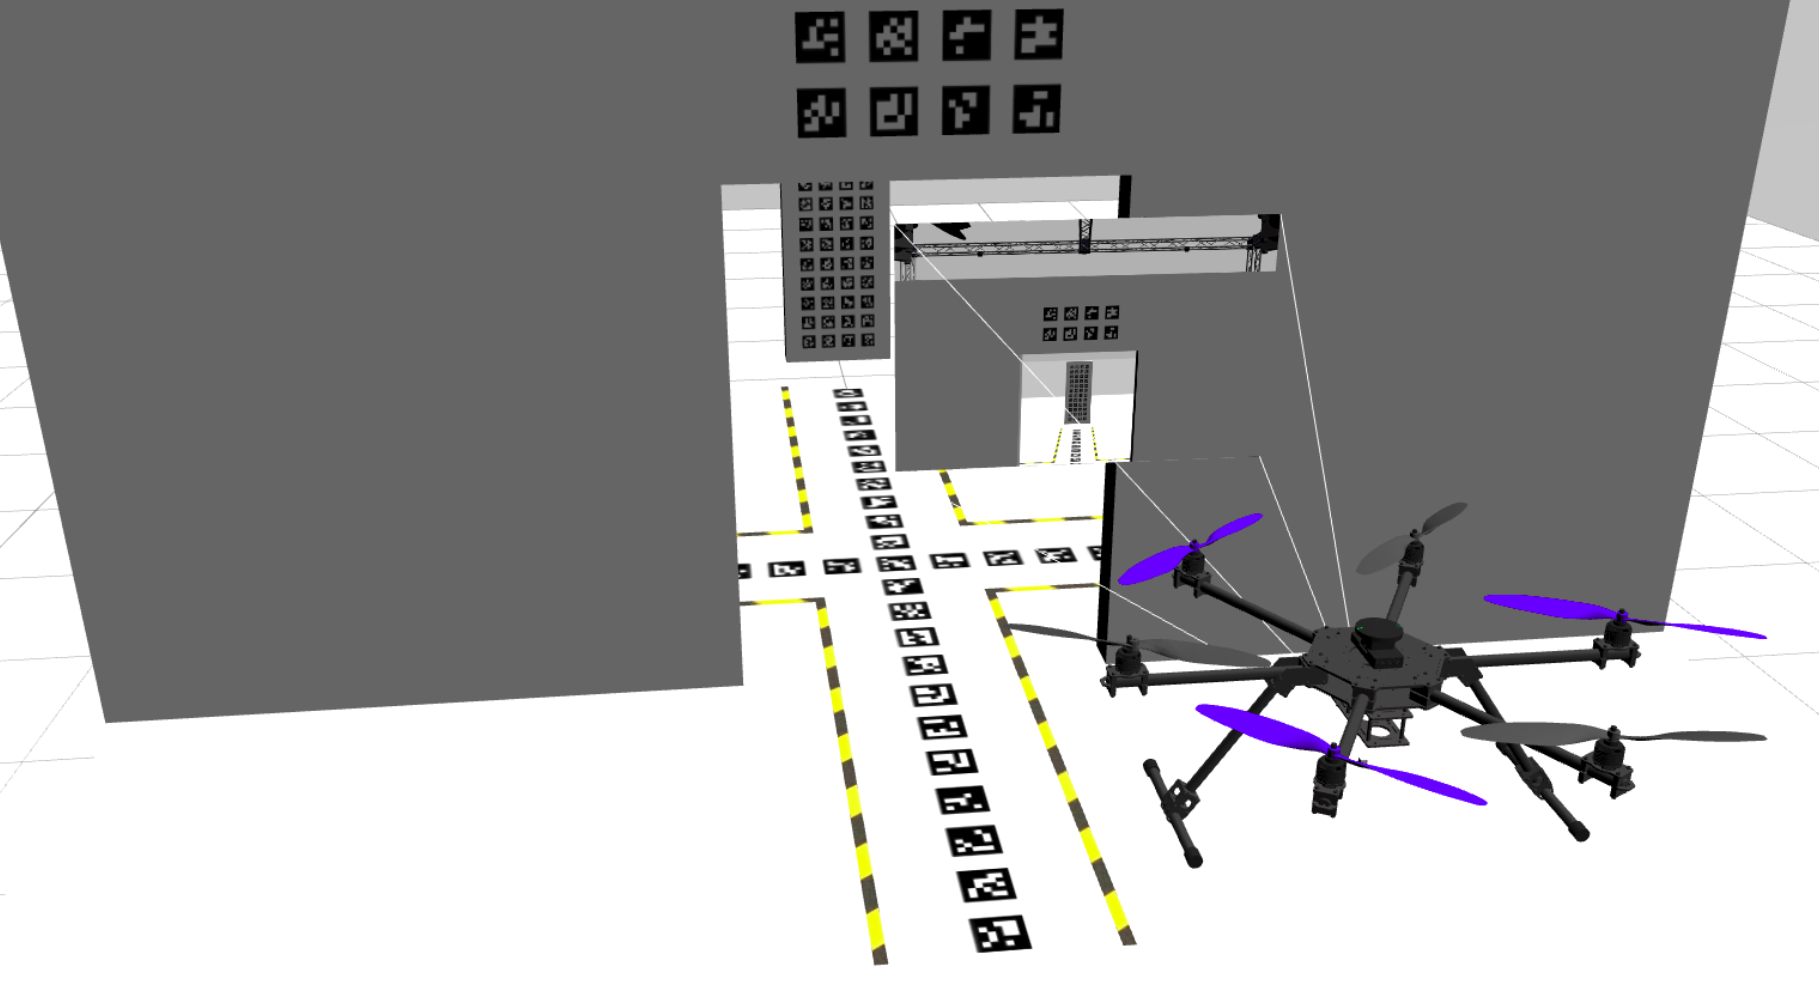
\includegraphics[height=3.3cm]{../Figures/img1.png}
           %\vspace{0.5em}
        \caption{}
        \label{fig:gps2vision_step1}
    \end{subfigure}
    %\hspace{5.0em}
    \begin{subfigure}[b]{.40\textwidth}
        \centering
        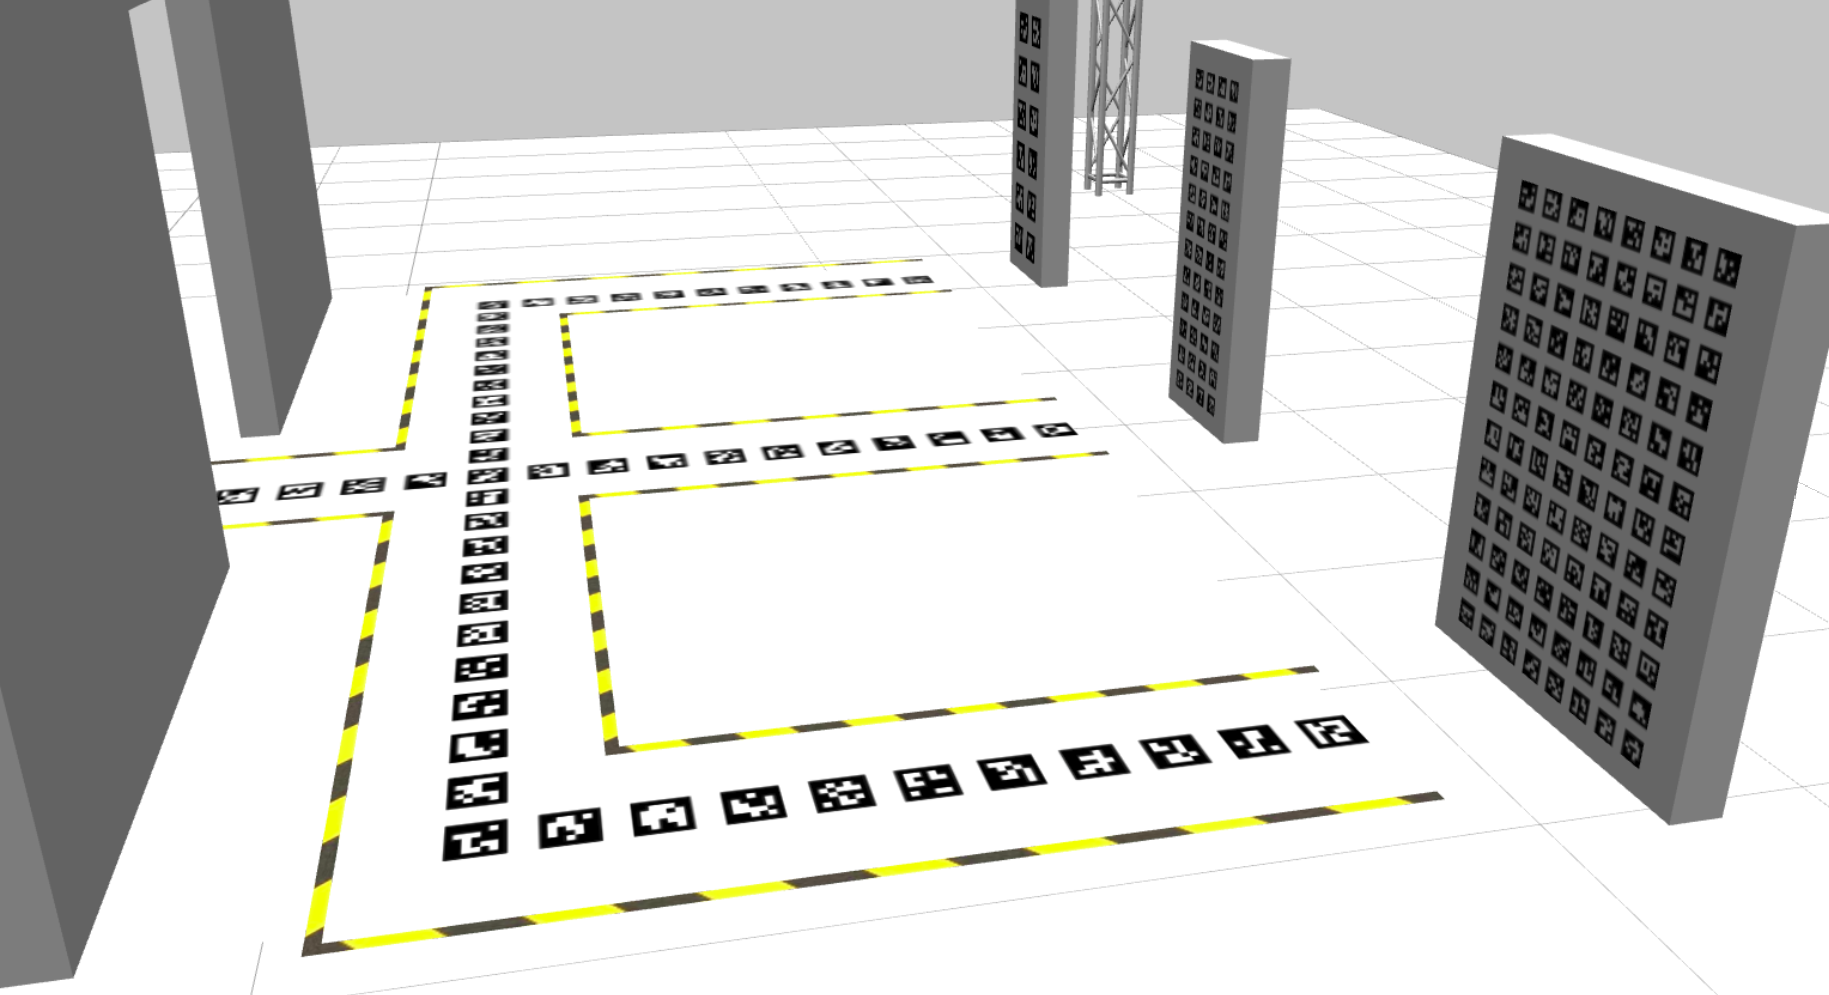
\includegraphics[height=3.3cm]{../Figures/img2.png}
        \caption{}
        \label{fig:gps2vision_step2}
    \end{subfigure}
    \caption{Illustration of the procedures in the GPS to vision based navigation. Initially the UAV uses GPS as navigation to a predefined location. Then it finds and navigates to the ArUco marker board located on the wall as seen in Figure \ref{fig:gps2vision_step1} using its front camera. When close enough to the board located on the wall, the UAV will start using the bottom camera for vision based navigation according to the markers located on the ground. Now the UAV can move to the indoor environment for recharging and land in front of one of the three landing ArUco marker boards as seen in Figure \ref{fig:gps2vision_step2} where the UAV again will use the front camera for detecting the ArUco marker landing boards} 
    \label{fig:gps2vision_steps}
\end{figure}

A solution to this problem could be to attach cameras on the UAV and analyze the incoming data using computer vision. By placing markers on the ground, the position of these markers could be found with high accuracy and precision. This would enable autonomous flight tasks where high accuracy and precision of the position is needed.      

This project proposes methods for navigation in environments using computer vision. The basic idea of this can be seen in Figure \ref{fig:gps2vision_steps}. Here the UAV will fly autonomously using GPS coordinates until the UAV has to move inside a vision navigation area for recharging. The UAV will use the ArUco marker board located on the wall for the actual GPS to vision transition and afterwards using the markers located on the ground for the navigation using vision in the indoor environment. Then an acurate and precise landing can be executed using the ArUco marker landing boards from where the recharging is to take place. This is a cheap and effective solution when lack of GPS is present e.g using low cost GPS systems or inside buildings \cite{Visual-Inertial-Navigation}. 

The robot operating system (ROS) will be used along the PX4 autopilot in order to achieve autonomous flight of the UAV with Gazebo as the simulation environment so that the UAV can be sufficiently tested before flying. 

\subsection{Related work}
\label{sec:related_work}

Vision based navigation is a vast research area for utilizing computer vision for navigation and precision landings. According to \cite{OnBoardVisionAutonomousLanding}, landing platforms can be categorized into the three groups for different landing scenarios. \textit{Category one} defines platforms which are fixed, \textit{category two} for moving platforms of two degrees and \textit{category three} which considers landings on ships where the platform of the ship deck can be modeled as a rigid body with six additional degrees of freedom based on the psychical movements of the waves. 

Fixed based platforms using computer vision have been used for some time to enable landings for better accuracy compared to that of using GPS. In \cite{AVisionBasedSystemForAutonomousVerticaLanding}, an implementation of using ArUco markers located on the landing platform is proposed. Here the UAV is able to land and recognize the ArUco marker located on the ground from an altitude of twenty meters using Pixhawk 4 as flight controller with a Raspberry Pi 3 for onboard computing. 

In \cite{AutonomousRechargingSystemforDronesOne} \cite{AutonomousRechargingSystemforDronesTwo} autonomous landings are performed where the UAV is to land on a wireless charging station. However, though these systems perform quite well, both use a single ArUco marker for pose estimation with a cost in reduced accuracy which may affect the overall performance of the landing system. The advantage of using more markers for pose estimation was investigated by Tiago Gomes Carreira \cite{QuadcopterAutomaticLandingOnaDockingStation}. He performed an evaluation in using different sets of ArUco markers for where the error in the estimation is based on one, four and eights ArUco markers. Results shows performance improvements when more markers are present in the image. 

Shifeng Zhang et al. \cite{AnOnboardVisionBasedSystemNovelLandingPad} 	proposes a different method where more than one ArUco marker is used in the vision based landing. In this setup a landing platform with ArUco markers with different sizes is used. This was found to make the system more reliable when the pose estimation of the markers is made from different distances.   

Instead of only using a camera attached to the UAV which points downwards, Ghader Karimian et al. \cite{AutomaticnavigationandlandingofanindoorAR} presented a method for using both a bottom-facing and front-facing camera to utilize automatic navigation and landing of a UAV in indoor environments.  This solution uses a single ArUco marker and IMU measurements to be fused in a Kalman filter. In this setup, the UAV will use the front camera to navigate towards a marker located on the ground. When the UAV loses sight of the marker using the front camera, it will continue in the same direction using IMU data until the marker is visible from the perspective of the bottom camera where it is to land.

For vision based navigation in indoor inviroments Chouaib Harik et al. \cite{TowardsAnAutonomousVisionBasedInventoryDroneOne} proposed a solution by having an Unmanned Ground Vehicle (UGV) to be used as platform for the UAV. Here the platform contains a marker from which the UAV can takeoff and land. This UGV can navigate among rows of racks where the UAV takes off and scans the inventories where it keeps its pose using sensor fusion of IMU and marker data. However, this solution requires an UGV equipped with lidars for navigation which is expensive. 

Another method was proposed by Michael Maurer et al. \cite{TowardsAnAutonomousVisionBasedInventoryDroneTwo}. This method uses model-based visual localization to that of a precomputed
map of the environment which is used to estimate the drift of a odometry sensor to achieve centimeter precision of the pose of the UAV. Both these methods yields solutions to vision based navigation for indoor environments, but does not take into account ways of making transitions between using GPS and vision as navigation.

The way this thesis differs from previous work is the implementation of a GPS to vision based transition using the front-facing camera of the UAV to navigate to an ArUco marker board located on the wall. Moreover, this implementation will be build on a completely autonomous system, where the UAV can handle the transition of using GPS, then vision, land and then move out of the vision navigation area for then again to use GPS for mission executions.
  
\newpage
\subsection{Problem Statement}

The UAV must be able to make a reliable GPS to vision transition. This leads to the challenge of finding a robust solution for the transition of using GPS coordinates to indoor vision based navigation even in windy conditions. This transition must be incorporated using markers located on the wall to the entrance of the vision navigation area. The UAV then needs to be capable of navigating in indoor environments using markers located on the ground.    

A solution for onboard computing for pose estimation of the markers as well as autonomous flight must be found. This says that the computer must be able to perform real-time calculations of the pose of the markers to insure a reliable system. 

Furthermore, the precise landing should be implemented in such a way that the time, from which the UAV is hovering above the marker to the landing is performed, is minimized. The same goes for the error associated with the precision landing .  

This leads to the following problems:

\begin{itemize}
    \item How can computer vision be used to detect markers?
    \item How can a smooth transition between using GPS coordinates to vision based navigation be found?
    \item How can navigation between markers be performed?
    \item How can sensor fusion be implemented for pose optimization?
    \item How can a precise landing be executed?
    \item How can the landing time be reduced without causing instabilities to the UAV?
    
\end{itemize} 

\subsection{Specification of requirements}

From the outline of the project as well as the problem statement, the following requirements for the project have been formulated:

\begin{itemize}
	\item The implemented system must be able to function completely autonomous
    \item The error of the landing must not exceed $\pm 10$ cm. 
    \item The pilot must be able to send missions on a wireless connection to the UAV for execution
    \item The UAV should be able to make the transition of using GPS coordinates to indoor vision based navigation even in windy conditions i.e up to 8 m/s.
    \item The landing must be performed within 5 seconds from where the UAV is hovering 1.5 meters above the landing sight to a landing is performed

\end{itemize}


\newpage
\subsection{Tentative time schedule}
\label{sec:tentative_time_schedule}

At the start of the project a tentative time schedule was formulated. This was done to keep an overview of the most essential elements which had to be implemented. Time was put aside to complete each block of work so that things could be done in an order which was found appropriate.  This time schedule can be seen in Figure \ref{fig:Tentative_time_schedule_2020} and \ref{fig:Tentative_time_schedule_2021}. The main focus has been to get things to work properly in simulations before conducting any tests on the drone to reduce the risks of failures.   

\newcounter{myWeekNum}
\stepcounter{myWeekNum}
%
\newcommand{\myWeek}{\themyWeekNum
    \stepcounter{myWeekNum}
    \ifnum\themyWeekNum=53
         \setcounter{myWeekNum}{1}
    \else\fi
}

\setcounter{myWeekNum}{36}
\ganttset{%
calendar week text={\myWeek{}}%
}
%
\begin{figure}[h!bt]
\begin{center}

\advance\leftskip-2.0cm

\begin{ganttchart}[
vgrid={*{6}{draw=none}, dotted},
x unit=.08cm,
y unit title=.7cm,
y unit chart=.44cm,
time slot format=isodate,
time slot format/start date=2020-09-01]{2020-09-01}{2020-12-27}
\ganttset{bar height=.6}
\gantttitlecalendar{year, month=name, week} \\
\ganttbar[bar/.append style={fill=blue}]{Simulation (Gazebo)}{2020-09-15}{2020-11-30}\\

\ganttbar[bar/.append style={fill=green}]{CAD modelling}{2020-09-01}{2020-09-14}\\

\ganttbar[bar/.append style={fill=red}]{ROS implementation}{2020-09-08}{2020-10-05}\\

\ganttbar[bar/.append style={fill=yellow}]{Computer vision}{2020-09-22}{2020-12-07}\\

\ganttbar[bar/.append style={fill=gray}]{Flight tests}{2020-12-01}{2020-12-07}\\

\ganttbar[bar/.append style={fill=black}]{Report writing}{2020-12-08}{2020-12-14}
\ganttbar[bar/.append style={fill=black}]{}{2020-11-24}{2020-11-30}
\ganttbar[bar/.append style={fill=black}]{}{2020-11-10}{2020-11-16}
\ganttbar[bar/.append style={fill=black}]{}{2020-10-27}{2020-11-02}

\end{ganttchart}
\caption{Tentative time schedule for 2020}
\label{fig:Tentative_time_schedule_2020}
\end{center}

\end{figure}

In the initial phase of the project CAD models were created for buildings and markers. Then the ROS implementation along the PX4 software was installed which would be used in the simulation. Hence, the main focus of the project for 2020 was the computer vision part where marker detection, pose estimation, navigation between markers and landing was in focus which was programmed in python with OpenCV as the computer vision software. These used methods will be discussed in Section \ref{sec:methods}. 

In the second part of the project, the initial idea was to test the implementation on the real hardware. This was scheduled to begin in the start of March. However, due to the current situation with Covid-19, this was not possible because all access to Hans Christian Andersen airport in Odense was rejected. Due to these limitations, more work has been put into the simulations. As seen in Figure \ref{fig:Tentative_time_schedule_2021}, approximately two months were put aside for flight tests. Because of the limitations just discussed, this period of time had now been used for simulations instead.    

\setcounter{myWeekNum}{5}
\ganttset{%
calendar week text={\myWeek{}}%
}
%
\begin{figure}[h!bt]
\begin{center}

\advance\leftskip-2.0cm

\begin{ganttchart}[
vgrid={*{6}{draw=none}, dotted},
x unit=.08cm,
y unit title=.7cm,
y unit chart=.44cm,
time slot format=isodate,
time slot format/start date=2021-02-01]{2021-02-01}{2021-05-30}
\ganttset{bar height=.6}
\gantttitlecalendar{year, month=name, week} \\

\ganttbar[bar/.append style={fill=blue}]{Simulation (Gazebo)}{2021-02-01}{2021-02-28}\\

\ganttbar[bar/.append style={fill=yellow}]{Computer vision}{2021-02-01}{2021-03-28}\\

\ganttbar[bar/.append style={fill=gray}]{Flight tests}{2021-02-29}{2021-05-02}\\

\ganttbar[bar/.append style={fill=black}]{Report writing}{2021-05-03}{2021-05-30}
\ganttbar[bar/.append style={fill=black}]{}{2021-03-22}{2021-03-28}
\ganttbar[bar/.append style={fill=black}]{}{2021-04-05}{2021-04-11}
\ganttbar[bar/.append style={fill=black}]{}{2021-04-19}{2021-04-25}
\end{ganttchart}
\end{center}
\caption{Tentative time schedule for 2021}
\label{fig:Tentative_time_schedule_2021}
\end{figure}

The result of the implementation of the autonomous system for offboard control was completed at the beginning of April where videos of all the tests in simulation were recorded for easy visualization of the procedures for testing the system. These can be seen by accessing the links from the results in Section \ref{sec:results}. 

Report writing has been done in small steps throughout the period of the project, but the main contribution to this part was done in May where the complete implementation of the system could be documented. 


\end{document}